%%%%%%%%%%%%%%%%%%%%%%%%%%%%%%%%%%%%%%%%%
% Presentation Poster
% Madrid 2017
%%%%%%%%%%%%%%%%%%%%%%%%%%%%%%%%%%%%%%%%%
%%%%%%%%%%%%%%%%%%%%%%%%%%%%%%%%%%%%%%%%%
%	Credits: 
%Jacobs Landscape Poster
% LaTeX Template
% Version 1.1 (14/06/14)
%
% Created by:
% Computational Physics and Biophysics Group, Jacobs University
% https://teamwork.jacobs-university.de:8443/confluence/display/CoPandBiG/LaTeX+Poster
% 
% Further modified by:
% Nathaniel Johnston (nathaniel@njohnston.ca)
%
% This template has been downloaded from:
% http://www.LaTeXTemplates.com
%
% License:
% CC BY-NC-SA 3.0 (http://creativecommons.org/licenses/by-nc-sa/3.0/)
%
%%%%%%%%%%%%%%%%%%%%%%%%%%%%%%%%%%%%%%%%%

%----------------------------------------------------------------------------------------
%	PACKAGES AND OTHER DOCUMENT CONFIGURATIONS
%----------------------------------------------------------------------------------------

\documentclass[final,20pt]{beamer}

\usepackage[scale=1.45]{beamerposter} % Use the beamerposter package for laying out the poster

\usepackage[multisym, geomec, basic, diffgeo]{./toninus-math-symbols}
	\renewcommand{\AffDualJet}{ J^{1 \TwistedAffine}E }
	\renewcommand{\LinDualJet}{ \overrightarrow{J^{1 \TwistedLinear}E} }

\usetheme{confposter} % Use the confposter theme supplied with this template

\setbeamercolor{block title}{fg=ngreen,bg=white} % Colors of the block titles
\setbeamercolor{block body}{fg=black,bg=white} % Colors of the body of blocks
\setbeamercolor{block alerted title}{fg=white,bg=dblue!70} % Colors of the highlighted block titles
\setbeamercolor{block alerted body}{fg=black,bg=dblue!10} % Colors of the body of highlighted blocks
% Many more colors are available for use in beamerthemeconfposter.sty

%-----------------------------------------------------------
% Define the column widths and overall poster size
% To set effective sepwid, onecolwid and twocolwid values, first choose how many columns you want and how much separation you want between columns
% In this template, the separation width chosen is 0.024 of the paper width and a 4-column layout
% onecolwid should therefore be (1-(# of columns+1)*sepwid)/# of columns e.g. (1-(4+1)*0.024)/4 = 0.22
% Set twocolwid to be (2*onecolwid)+sepwid = 0.464
% Set threecolwid to be (3*onecolwid)+2*sepwid = 0.708

\newlength{\sepwidinternal}
\newlength{\sepwidexternal}
\newlength{\onecolwid}
\newlength{\onehalfcolwid}
\newlength{\twocolwid}
\newlength{\threecolwid}
\setlength{\paperwidth}{48in} % A0 width: 46.8in
\setlength{\paperheight}{36in} % A0 height: 33.1in
\setlength{\sepwidinternal}{0.036\paperwidth} % Separation width (white space) between columns
\setlength{\sepwidexternal}{0.012\paperwidth} % Separation width (white space) between columns
\setlength{\onecolwid}{0.22\paperwidth} % Width of one column
\setlength{\onehalfcolwid}{0.34\paperwidth} % Width of one column and one half
\setlength{\twocolwid}{0.464\paperwidth} % Width of two columns
\setlength{\threecolwid}{0.708\paperwidth} % Width of three columns
\setlength{\topmargin}{-0.5in} % Reduce the top margin size
%-----------------------------------------------------------

\usepackage{graphicx}  % Required for including images
\usepackage{booktabs} % Top and bottom rules for tables
\usepackage{marvosym}

%-----------------------------------------------------------
% Some shortcut
%-----------------------------------------------------------


%----------------------------------------------------------------------------------------
%	TITLE SECTION 
%----------------------------------------------------------------------------------------

\title{Multi-symplectic Geometry and application to modern Physics} % Poster title

\author{Antonio Michele Miti} % Author(s)

\institute{	Department of Mathematics and Physics, 
				Universit\`{a} Cattolica del Sacro Cuore, Brescia, Italy
				% and KU Leuven
				}% Institution(s)

%----------------------------------------------------------------------------------------

\begin{document}

\addtobeamertemplate{block end}{}{\vspace*{2ex}} % White space under blocks
\addtobeamertemplate{block alerted end}{}{\vspace*{2ex}} % White space under highlighted (alert) blocks

\setlength{\belowcaptionskip}{2ex} % White space under figures
\setlength\belowdisplayshortskip{2ex} % White space under equations

\begin{frame}[t] % The whole poster is enclosed in one beamer frame
\begin{columns}[t] % The whole poster consists of three major columns, the second of which is split into two columns twice - the [t] option aligns each column's content to the top


	\begin{column}{\sepwidexternal}\end{column} % Empty spacer column
	%----------------------------------------------------------------------------------------
	%	  FIRST COLUMN
	%----------------------------------------------------------------------------------------
	\begin{column}{\onecolwid} % The first column

		\begin{alertblock}{About Me}
			\begin{itemize}
				\item 
					1\textsuperscript{st}	year Ph.D student in Mathematics \\ 
					\emph{Joint International Ph.D. Program in Science}, 
					UCSC Brescia and KU Leuven.
				
				\item Master Degree in Physics with emphasis in Mathematical Physics
				\item \underline{Interests}:
					\begin{itemize}
						\item[-] Differential Geometry
						\item[-] Axiomatic Foundations of Physics
						\item[-] Geometric Mechanics of Field Systems
						\item[-] Geometric and Algebraic Quantization
						\item[-] Secondary calculus and cohomological physics
					\end{itemize}
				\item \underline{Supervisors}: 
					\begin{itemize}
						\item[-] Mauro Spera (UCSC)
						\item[-] Marco Zambon (KU Leuven)
					\end{itemize}
			\end{itemize}
		\end{alertblock}
		
		
		\vspace{0.5cm}
		\begin{block}{Research Project Objectives}
		\begin{itemize}
			\item\justifying Implement and explore the range of applicability of multi-symplectic and moment map methods in continuous media mechanics.
			\item\justifying Study the relations between the conserved quantities delivered from \emph{homotopy moment maps} and the notion of conserved charges stemming in classical and quantum field theory.
			\item\justifying Tackle the problem of \emph{symplectic reduction} in the general case. (The proper field-theoretic version of these notion is yet to be identified)
			\item\justifying Pursue the \emph{quantization commutes with reduction} program, started from the celebrated Guillemin-Sternberg conjecture, in the higher setting of multi-symplectic geometry.
			\item\justifying Contribute to setting up a precise \emph{mathematical characterization of classical fields} together with their quantum counterparts, in view of providing a solid foundation for both geometric and algebraic quantization schemes.
		\end{itemize}
		\end{block}


		\setbeamercolor{block alerted title}{fg=black,bg=norange} % Change the alert block title colors
		\setbeamercolor{block alerted body}{fg=black,bg=white} % Change the alert block body colors
		\vspace{1cm}
		\begin{alertblock}{Contact Information}
		\begin{center}
			\begin{tabular}{c c c}
				\ComputerMouse $\;$ &  \href{http://mastertoninus.github.io}{http://mastertoninus.github.io} & $\;$ \ComputerMouse \\
				\Letter $\;$ & \href{mailto:antoniomichele.miti@unicatt.it}{antoniomichele.miti@unicatt.it} & $\;$ \Letter
			\end{tabular}		
		\end{center}
		\end{alertblock}

	\end{column}


	\begin{column}{\sepwidinternal}\end{column} % Empty spacer column
	%----------------------------------------------------------------------------------------
	%	  SECOND COLUMN
	%----------------------------------------------------------------------------------------
	\begin{column}{\threecolwid} % Begin a column which is two columns wide (column 2)
		\begin{columns}[t,totalwidth=\threecolwid] % Split up the two columns wide column

			%-------------------------------------------------------------------------
			%  MULTISYMPLECTIC
			%-------------------------------------------------------------------------
			\begin{column}{\onehalfcolwid}\vspace{-.6in} % The first column within column 2 (column 2.1)
				\begin{block}{Multi-Symplectic Geometry}			
					\begin{figure}
						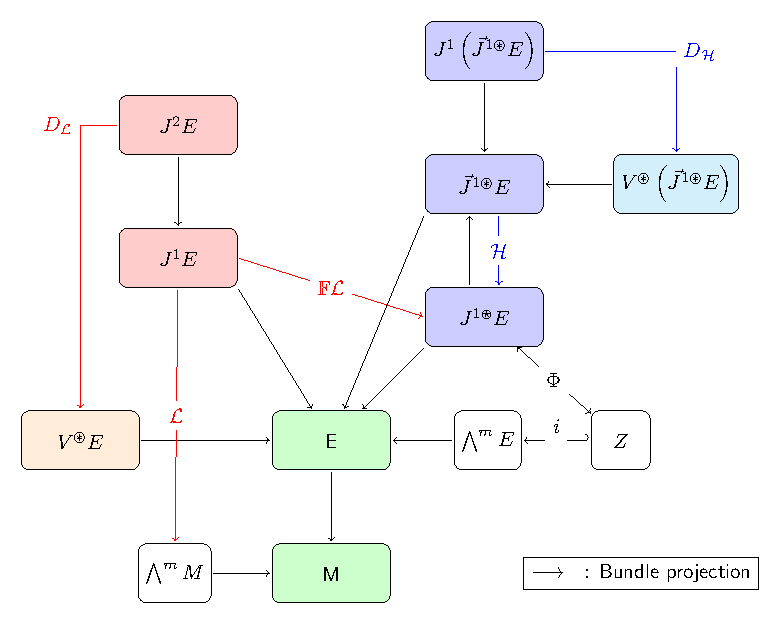
\includegraphics[height=32cm,keepaspectratio]{Pictures/Figure_ms_landscape}
						\caption{Multi-Symplectic landscape of classical field theories}
					\end{figure}

						Just as symplectic geometry is the natural arena for the classical mechanics of point-like systems, 
						multi-symplectic geometry encompasses field theories as well providing
						a powerful and unifying finite dimensional portrait suitable for the description of a rich variety of physical systems. 
						
						\vspace{1.5cm}
						\PointingHand \: \underline{Key Points} :
						\begin{itemize}
							\item \emph{Kinematics} is encoded by a finite dimensional smooth bundle $E = \left( E\rightarrow M \right)$ 
								called \emph{configuration bundle}.
							\item The first twisted affine dual bundle $J^{1 \TwistedAffine}E$, 
								carries a naturally defined form $\omega = -\textrm{d} \theta$, 
								obtained by pulling back the tautological $m$-form $\theta_\Lambda$ from $\bigwedge^m (E)$.\\
								It can be considered the theoretical analogue of the cotangent bundle in ordinary geometric mechanics.
							\item \emph{Dynamics} can be implemented by fixing a Lagrangian density $\Lagrangian$ 
										or an Hamiltonian density $\Hamiltonian$.
							\item The \emph{equations of motions} are encoded in the vector bundle maps $D_{\Lagrangian}$ or  $D_{\Hamiltonian}$
									whose action along holonomic sections is in encoded by pulling back the form $\omega$ 
									via a \emph{Legendre transformation}.
						\end{itemize}
							Abstracting, we are dealing with a manifold endowed with a closed and injective k-form ($2 \leq k < \textrm{dim}(M)$) 
							i.e.  a \emph{multi-symplectic manifold}.	
						
						
						


				\end{block}
			\end{column} % End of column 2.1

			\begin{column}{\sepwidinternal}\end{column} % Empty spacer column
			%-------------------------------------------------------------------------
			%  COVARIANT SYMPLECTIC APPROACH
			%-------------------------------------------------------------------------
			\begin{column}{\onehalfcolwid}\vspace{-.6in} % The second column within column 2 (column 2.2)
				\begin{block}{Covariant Symplectic Approach}	
					\begin{figure}
						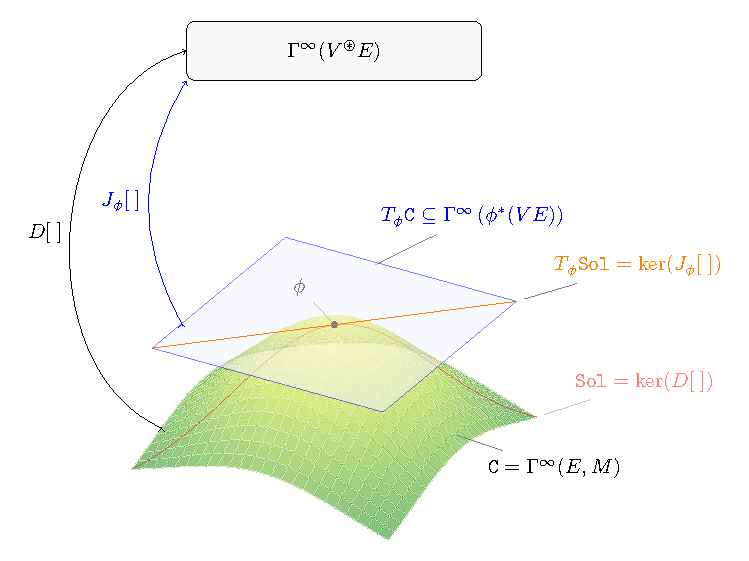
\includegraphics[height=32cm,keepaspectratio]{Pictures/Figure_Jacobi}
						\caption{Covariant-symplectic landscape of classical Lagrangian field theories}
					\end{figure}
					
					The transition to the \emph{(Covariant) Functional Approach} is basically a change of perspective,
					we have to move our attention from the bundles to the cross-sections on the bundles.
					%\footnote{The bundle to be considered depends on the dynamical picture employed, Lagrangian or Hamiltonian.}
					
					This imply that the central role will be played by an "infinite dimensional" manifold called  \emph{Covariant Phase Space}.

						\vspace{1.5cm}
						\PointingHand \: \underline{Key Points} :
						\begin{itemize}
							\item We call \emph{kinematic configurations} all the possible sections $\Conf \coloneqq \Gamma^\infty(E,M)$.
							\item Since operators $D_\Lagrangian$ and $D_\Hamiltonian$ are bundle-morphism, 
								They can be regarded as partial differential operators on $\Conf$ after composing them with the jet functor $j$.
							\item The collection of all the configurations solving the equation of motion takes the name of \emph{Covariant Phase space}
							 (here denoted by $\Sol$) .
							\item A remarkable feature of the $\Sol$ space is that it carries a naturally defined pre-symplectic form $\Omega$.\\
								That is a bilinear skew-symmetric form on each infinite dimensional vector space  $T_\phi\Sol$ which consists of those infinitesimal variations mapping a solution $\phi\in\Sol$ in another solution \emph{(Jacobi Fields)}.
						\end{itemize}
					
					An alternative construction is represented by the \emph{Peierls' brackets} which determine a Poisson structure on a suitable space of Lagrangian functionals.

					
				\end{block}
			\end{column} % End of column 2.1

		\end{columns} % End of the split of column 2 - any content after this will now take up 2 columns width
	\end{column}


\end{columns} % End of all the columns in the poster
\end{frame} % End of the enclosing frame
\end{document}



